\newpage
\subsection{Log systeem}
\subsubsection{Klassendiagram}
Om informatie over het programma op te slaan terwijl er metingen etc. gedaan worden kan er informatie naar één van de drie log bestanden geschreven worden. Er worden in totaal drie logbestanden bijgehouden: \emph{m\_Measurements}, \emph{m\_Log} en \emph{m\_Debug}. Er is een enum voor het type log dat we willen schrijven, in de implementatie zal hiervoor dan een herkenbare tag als prefix gezet worden voor de log entry. Er wordt ook gebruik gemaakt van een log scope, deze wordt gebruikt om aan te geven welk onderdeel van het programma iets naar het log geschreven heeft. Een scope zal een zelfde soort tag krijgen als het logtype.

\begin{figure}[H]
  \centering
  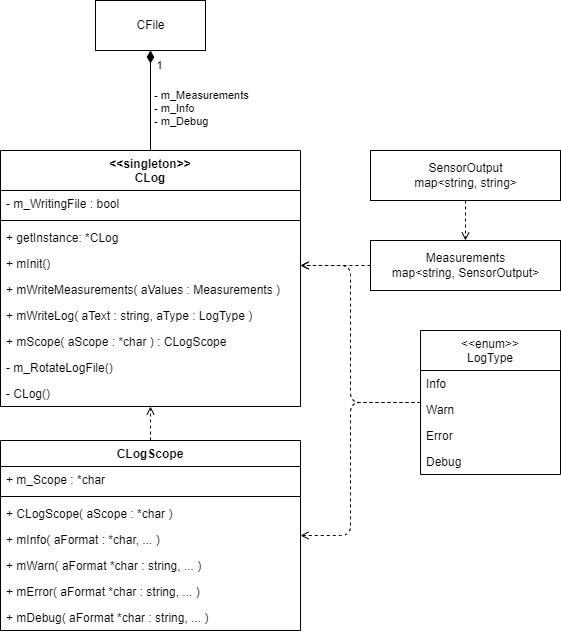
\includegraphics[width=.7\columnwidth]{uml/logger-abstraction.png}
\end{figure}

\newpage
\subsubsection{Toestandsdiagram}
Een nieuwe regel kan aan het log toegevoegd worden via twee verschillende functies. \emph{mWriteMeasurements()} en \emph{mWriteLog()}, de eerste hiervan wordt gebruikt om naar het log bestand in \emph{m\_Measurements} te schrijven wanneer er geen actieve internet verbinding is. De tweede kan zowel naar \emph{m\_Log} en \emph{m\_Debug} schrijven, afhankelijk van het \emph{LogType} dat wordt meegegeven in de functie. De \emph{LogType} wordt bepaald door de functie die wordt aangeroepen in \emph{CLogScope}.
\vspace{1em}
Wanneer er geen SD kaart in de SenseBox zit wordt dit verwerkt in de \emph{CFile} klasse en zal dit niet zorgen voor problemen in de \emph{CLog} klasse.

\begin{figure}[H]
  \centering
  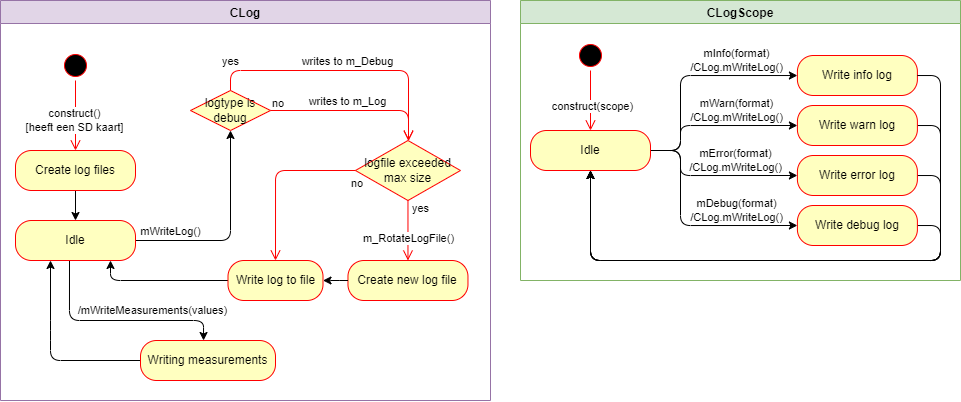
\includegraphics[width=\columnwidth]{uml/logger-state-diagram.png}
\end{figure}